\section{Lambda-Architektur}

\begin{quote}\glqq add quote \grqq~\cite[S.14]{Roth.2016}\end{quote} 
Bei der Verarbeitung von Big Data entstehen Herausforderungen wie z. B. die Echtzeitverarbeitung und die Hohe Rechenkomplexität. Um diese Herausforderungen zu bewältigen wird eine Big-Data-Architektur benötigt, welche eine geringe Latenz zwischen Ein- und Ausgabe aufweist. In diesem Kontext wird oft die Lambda-Architektur erwähnt. Diese besteht aus zwei Kernschichten: Batch- und Speed-Layer. Die Vereinigung dieser Schichten führt zu einer Echtzeitübermittlung der Daten. 
\begin{figure}[h!]
	\centering
	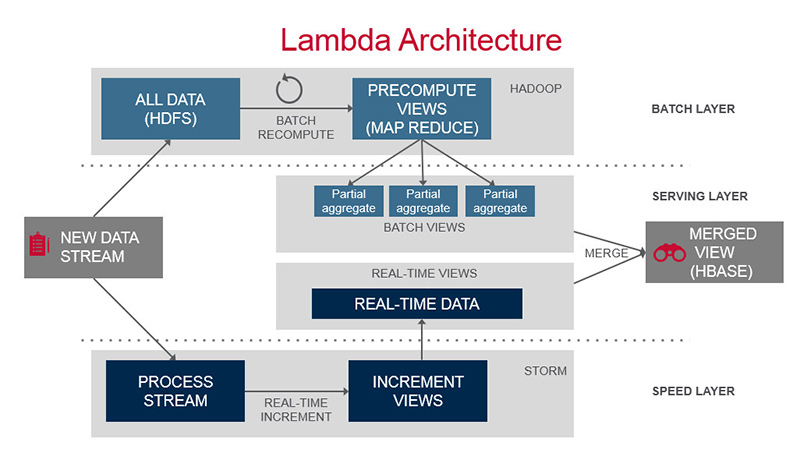
\includegraphics[width=1.0\linewidth]{images/lambda-architecture}
	\caption{Aufbau der Lambda-Architektur} %Generelle
	\label{fig:cnn_structure}
\end{figure}
\\ \textbf{Speed Layer}. Sie hat die Aufgabe möglichst aktuelle Daten zu liefern. Dabei wird nicht auf Datenvollständigkeit und -korrektheit geachtet, da die Datenmenge bei so einer hohen Frequenz nicht vollständig verarbeitet werden können bzw. dies nicht zwanghaft notwendig ist. Beispielsweise ein Sensor, der in Millisekunden abständen die Raumtemperatur verschickt. Hier könnte auch jeden tausendsten Sensorwert verarbeitet werden, da der Nutzwert von mehreren Daten an dieser Stelle nicht gegeben ist. Hier geht es darum, dass die Verzögerungslücke, welches von der Stapelschicht verursacht wird, zu minimieren. Die Verarbeitung der Daten geschieht im besten Falle komplett „in-Memory“.\\ \\ \textbf{Batch Layer}. Sie bezieht alle Daten ein und achtet darauf, exakte Ergebnisse zu erbringen. Im Gegensatz zu dem Speed Layer muss die Daten nicht im Speicher halten und kann Analysen mehrere Zeitfenster hinweg durchführen. Beispielsweise wäre ein Trainingsmodell aus dem Bereich „Machine Learning“ ein Anwendungsfall, welches Microsoft Azure ebenfalls unterstützt \cite{Berle.2017}. 

